\documentclass[a4paper]{article}  

\usepackage{mathtools}
\usepackage{amsthm}
\usepackage{amssymb}
\usepackage{tikz}
\usepackage{algpseudocode}

\title{CS270 Homework 1}
\author{Valkyrie Savage}

\begin{document}
\maketitle

\begin{enumerate}
\item Routing and Fractional Flow
	\begin{enumerate}
	\item Following is a simple example of a graph in which the maximum congestion in optimal solutions to the path routing problem and the fractional flow problem differ, with the solution to the \textbf{path routing} on the left and the solution to the \textbf{fractional flow} on the right.
		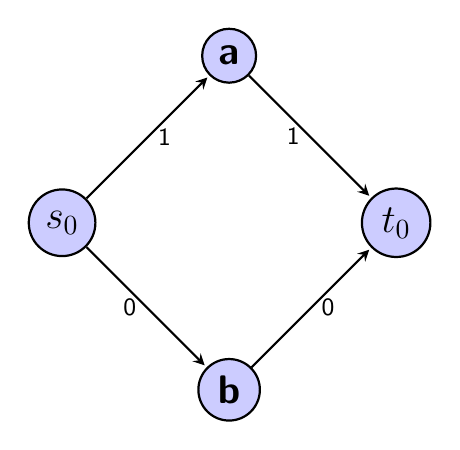
\begin{tikzpicture}[->,>=stealth,shorten >=1pt,auto,node distance=3cm,
 		thick,main node/.style={circle,fill=blue!20,draw,font=\sffamily\Large\bfseries}]

  		\node[main node] (B) {a};
  		\node[main node] (A) [below left of=B] {$s_0$};
  		\node[main node] (C) [below right of=A] {b};
  		\node[main node] (D) [below right of=B] {$t_0$};

  		\path[every node/.style={font=\sffamily\small}]
    		(B) edge node [left] {1} (D)
    		(A) edge node [right] {1} (B)
        		edge node [left]  {0} (C)
    		(C) edge node [right] {0} (D);
		\end{tikzpicture}
		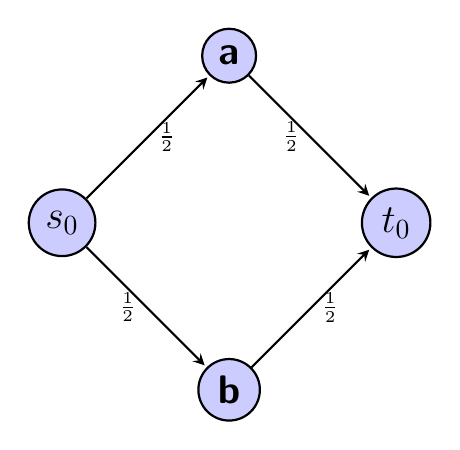
\begin{tikzpicture}[->,>=stealth,shorten >=1pt,auto,node distance=3cm,
 		thick,main node/.style={circle,fill=blue!20,draw,font=\sffamily\Large\bfseries}]

  		\node[main node] (B) {a};
  		\node[main node] (A) [below left of=B] {$s_0$};
  		\node[main node] (C) [below right of=A] {b};
  		\node[main node] (D) [below right of=B] {$t_0$};

  		\path[every node/.style={font=\sffamily\small}]
    		(B) edge node [left] {$\frac{1}{2}$} (D)
    		(A) edge node [right] {$\frac{1}{2}$} (B)
        		edge node [left]  {$\frac{1}{2}$} (C)
    		(C) edge node [right] {$\frac{1}{2}$} (D);
		\end{tikzpicture}\\
	\item This problem is very similar to proving the toll problem is the lower bound on the optimal solution to the path routing problem, so we will use similar conventions: $p_{ij}$ is a flow connecting $(s_i, t_i)$, and we will let the set of all such flows be $P_i = \{p_{ij}\}$.  $c(e)$ is the congestion on edge $e$ under the routing, being in this case the sum of the fractional path flows using that edge.  The length of $p_{ij}$ is $d(p_{ij})$.  Let the fractional flow of $p_{ij}$ equal $f_{ij}$.  We proceed as in the integral problem, but the crux is that the lengths of the edges in a path do not necessarily add up to $1$: however, the sum of all the paths $p_{ij}$ connecting $(s_i, t_i)$ does.
		\begin{align*}
			max_{e \in E} c(e) & \geq \sum_{e \in E} c(e) d(e) \\
			&= \sum_{e \in E} d(e) \sum_{i} \sum_{j:p_{ij} \ni e} f_{ij} \\
			&= \sum_{e \in E} \sum_{i} \sum_{j:p_{ij} \ni e} f_{ij} d(e) \\
			&= \sum_{i} \sum_{j} \sum_{e \in p_{ij}} f_{ij} d(e) \\
			&= \sum_{i} \sum_{j} f_{ij} \sum_{e \in p_{ij}} d(e) \\
			&= \sum_{i} \sum_{j} f_{ij} d(p_{ij}) \\
			&\geq \sum_{i} min_{j} d(p_{ij}) \\
			&= \sum_{i} d(s_i, t_i) \\
		\end{align*}
		Thus the toll problem is a lower bound on the fractional flow routing problem.
	\end{enumerate}
\item Equilibrium - pondered and completed but not written up.
\item Maximum weight matching vs. minimum weight vertex cover
	\begin{enumerate}
	\item Given $M$ a solution to the maximum weight matching problem and $p(\cdot)$ a solution to the minimum price vertex cover: $M=p(\cdot)$ iff the edges in the matching are tight, the price function is feasible, and there is a perfect matching.  All of these are satisfied, $\therefore M=p(\cdot)$.  When we increase the weight of an edge $(u,v)$ in our bipartite graph by $\delta$, we begin by adjusting $p(u)$ to $p(u) + \delta$.  If $(u,v) \in M$, then we are done.

	Otherwise, we have made one edge in our matching not tight.  Let this edge be $(u,v_1)$.  We adjust $p(v_1)$ to $p(v_1) - \delta$ to keep it tight.  Now we may have made one or more edges infeasible.

	We will maintain a global priority queue $Q$ containing edges in order of most infeasible to least infeasible.  We start at $v_1$, and put all edges $(u_i,v_1) : u_i \neq u$ in $Q$.  We pull the first edge, $(u_i,v_1)$ off $Q$ and adjust $p(u_i)$ to $p(u_i) + \epsilon$, where $\epsilon$ is the minimum adjustment we need to make to make the edge feasible.  Also note that $\epsilon \leq \delta$, and since we are maintaining our $Q$ in feasibility order we will eventually get to $\epsilon = 0$.

	We continue, since we have again made edges in our matching not tight, and then we adjust again to make edges feasible.  When we arrive at a vertex $v_j : (u, v_j) \in E$, we have made a cycle.  We flip all edges traversed in this cycle: that is, edges that were not matched previously are matched, and edges that were matched previously are no longer matched.  On the other hand, when we arrive at a vertex $v_k$ where $\forall u_i, (u_i, v_k) \in E, p(u_i) + p(v_k) = w(u_i, v_k)$, we have reached an end and do not need to flip the edges we adjusted along the way.

	In either case, then we return to $Q$, and pull off the next most infeasible edge, wherever it is.  We continue thusly until $Q$ is empty, in which case we are done.

Given $m$ the edges and $n$ the vertices, the runtime of this algorithm is $O(mlogm)$.  We traverse each edge in the graph at most once (thanks to our handy priority queue) which is $O(m)$, and we maintain the priority queue of the most infeasible edges which is $O(logm)$.
	\item We can apply the above algorithm to the entire matching problem by starting with 0-weight edges everywhere and some arbitrary matching (as long as it is perfect).  We can then increase the weight of one edge at a time to the correct weight, running our algorithm each time.  In this case, the running of our algorithm would be $O(m^2logn)$ for the full matching problem.
	\end{enumerate}
\end{enumerate}
\end{document}